% Chapter Template

\chapter{Methods} % Main chapter title

\label{Methods} % Change X to a consecutive number; for referencing this chapter elsewhere, use \ref{ChapterX}

%----------------------------------------------------------------------------------------
%	SECTION 1
%----------------------------------------------------------------------------------------

Sound is the propagation of waves of pressure through a medium. When a gun is fired, the vibrations produced alternately compress and rarefy the medium, leading to waves of high and low pressure that propagate in all directions \citep{Bradbury2011}. Over time and distance, these waves attenuate, their amplitude reducing as energy dissipates into the environment \citep{Russ2013}. The sound waves can then be transduced into an electrical signal.  To record digitally, the analogue signal is sampled at a certain rate (typically measured in thousands of samples per second, kHz) and bit-depth (number of possible amplitude levels, typically 16-bit), with both parameters being important for determining frequency and amplitude resolution respectively. The signal information is then electronically recorded in the time-amplitude domain and can be processed mathematically using a fast Fourier transform (FFT) to convert the amplitude data into frequency data \citep{Fourier1822, Cooley1964}. For a given time window in the recording, the FFT calculates the frequency components of the signal and their relative amplitudes, producing a frequency spectrum. For a visual representation of the whole recording, an FFT is calculated with an overlapping short sliding window across the length of the recording, producing a spectrogram \citep{TheRoy2003} This entire process is outlined in Figure ~\ref{fig:audio_analysis}.\\

\begin{figure}
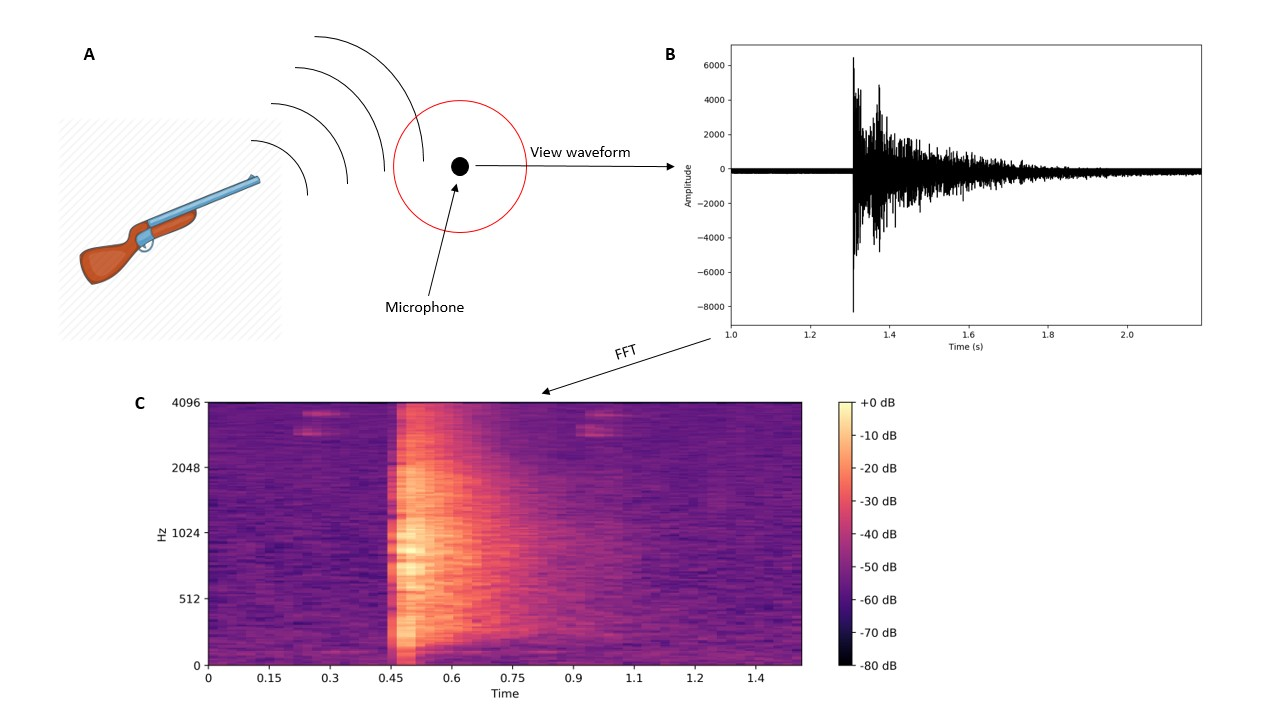
\includegraphics[width=1.2\textwidth,center]{Figures/audio_analysis}\caption[Analysis of acoustic data]{Recording and analysis of an acoustic signal. The emitted sound is transduced into an electrical signal by a microphone (\textbf{A}). In digital recording, the sound can be reconstructed in the time-amplitude domain (\textbf{B}) using the specified sampling rate (kHz). A frequency spectrum can then be produced using a fast Fourier transform (FFT), which calculates the signal’s frequency components and their relative amplitudes. Calculating FFT within a sliding window across the recording produces a spectrogram, with time on the x-axis, frequency on the y-axis, and with amplitude (energy) shown as colour intensity (\textbf{C})}\label{fig:audio_analysis}
\end{figure}

\noindent It is common in audio classification to plot a variant of the traditional spectrogram: the mel-frequency spectrogram. This involves calculating the mel-frequency cepstrum (MFC) which is a representation of the sound's power spectrum after the frequency has passed through a mathematical function. Mel-frequency cepstral coefficients (MFCCs) are the constituent coefficients of an MFC \citep{Xu2004}. They are calculated from a cepstral representation of the sound, with frequency bands equally spaced on the mel scale \citep{Stevens1937}. Spectrograms are fundamental to the analysis of acoustic data as they allow very specific sounds, such as a spider monkey call or a gunshot, to be visually identified and labelled, either manually or automatically.

\section{Data collection and preprocessing}


\subsection{Study site}

The audio data used in this study was collected at a study site in the Osa Peninsula, Costa Rica (Figure ~\ref{fig:peninsula_map}). This 2,500 km$^2$ site sits in a particularly diverse region, containing approximately 2.5\% of the world's species on less than 0.001\% of its land area \citep{Lawson2019}. Three national parks - Corcovado, Piedras Blancas, and the Terreba-Sierpe wetlands - and one forest reserve are represented within this study site. There has been significant landscape alterations in these areas which are inevitably brought about by an expanding human population and the introduction of agriculture and urbanisation \citep{Hobinger2012}.

\begin{figure}
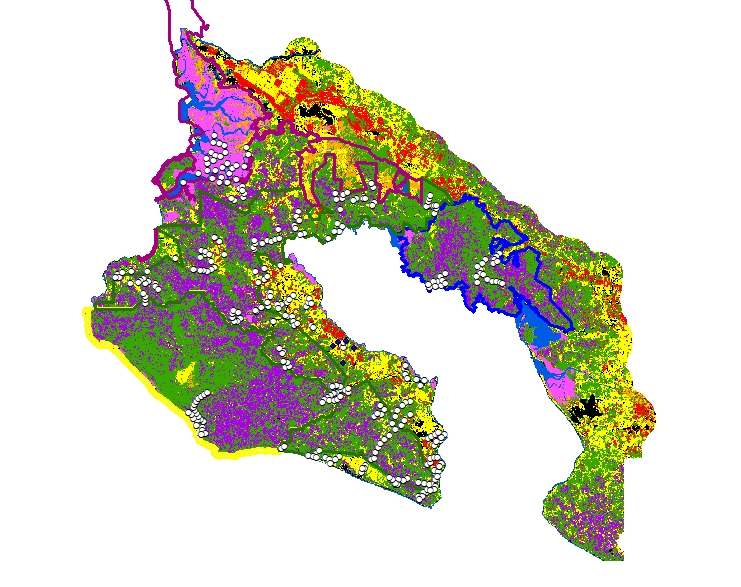
\includegraphics[width=1.2\textwidth,center]{Figures/peninsula_map}\caption[Map of Osa Peninsula]{Map of the study site in the Osa Peninsula \cite{Lawson2019} (NEED KEY/AREAS MARKED)}\label{fig:peninsula_map}
\end{figure}

\subsection{Sampling}

In this study, data from six AudioMoth acoustic sensors were collocted over six consecutive days, totalling 960 hours. These sensors covered protected forest reserve, protected grassland, and unprotected forest (TABLE), and were placed in areas known to be hotspots for hunting (personal communication, Jenna Lawson). Each device was set to record for three periods a day, 0500-0930, 1400-1830, and 2100-0300. These periods were chosen to coincide with the peak activity levels of \textit{A. geoffroyi} and their associated poaching. Sound was recorded continuously during these periods at a sample rate of 48 kHz and the devices were contained in waterproof casing to avoid damage. Every minute of audio data was saved in a separate file with the filename being a Unix hexadecimal timestamp. Where possible, trails and other areas of high human density were avoided.


\subsection{Training data}

\cite{Hill2018} provided the labelled audio data which was used in their study and was used in this study to train the neural network. The data was collected using 36 AudioMoth devices in the tropical rainforests in Pook's Hill Reserve, Belize. The devices covered 13 sites and were placed 200 m apart from each other. Controlled gunshots were set off by the research team and were labelled as positives in the dataset through visual inspection of spectograms. The detection algorithms used were able to detect 66\% of gunshots up to 500 m away and 50\% up to 1 km away. Devices facing towards the gunshot were 80\% more likely to detect it than those facing away.



\section{Machine learning}

All coding in this study was carried out using either Python (3.6.8) or bash (4.4.20), on an Ubuntu (18.04.3) operating system. For the training data, each audio file was split into four second clips using the pydub (0.23.1) Python module. Each clip was then plotted as a 60x60 mel-spectrogram using the librosa (0.7.0) Python module.\\

\noindent The CNN was then trained using the Keras (2.2.4) Python module. Mel-spectrogram images were imported and the pixel values were normalised to take values between 0 and 1 (rather than 0 and 255) as this has been shown to improve convergence and stability \citep{Liao2016}. The data was split randomly into training and validation data in the ratio 3:1 as this has been shown to be appropriate for a dataset of this size \citep{Guyon1997}. The seed for random number generation was set to ensure repeatability.

\subsection{Convolutional Neural Network}

The CNN was constructed using \cite{Chollet2016}'s tutorial as a template. The first layer was a convolutional 2D kernel which was convolved with the input layer to produce a tensor of outputs, the input layer being $n$ spectrograms of 64x64x3 size. It contained 32 nodes which determines the dimensionality of the output space and a 3x3 convolutional window. A 'relu' activation function was then applied as this was shown by \cite{Glorot2011} to enable better training of deep neural networks, compared to other common activation functions such as the logistic sigmoid. The identified features are then passed through a max pooling layer which determines the most activated presence of each feature within a 2x2 cluster of features. Essentially, this filters out the less important features and keeps the most important ones to be passed to the next layer. In this model, these first three layers were repeated in the same order two further times, with the model then totalling nine layers. The features were then passed to a 'flattening' layer. This is a layer that takes a two-dimensional matrix of features and transforms them into a vector of features that can be fed to a neural network classifier, in this case a 'dense' layer composed of 64 fully-connected neurons. These neurons linearly take all the inputs from the previous layer, apply a weight to them and output to the next layer which, in this CNN, was another 'relu' activation layer. The activation layer output was then passed through a 'dropout' layer. In this case, that involved randomly discarding 50\% of nodes in an effort to minimise overfitting. The remaining nodes were put through another 'dense' layer, this time with 2 nodes as this CNN was only being trained in a binary 'gunshot' or 'no gunshot' manner. The output of this 'dense' layer was passed through a final 'softmax' activation layer which is similar to logistic regression but usually used in multi-classification problems. However, it has been shown to be more effective than logistic regression, even in binomial classification (FIGURE NEEDED).

\subsection{Training and testing the model}
Initially, I trained the model for 100 epochs on the data provided by \cite{Hill2018} by randomly splitting the data into training and test data in a ratio of 70:30. The training and test data was comprised of equal numbers of positive (gunshot present) and negative (gunshot not present) spectra as imbalanced ratios have been previously shown to be ineffective \citep{Kim2018} and preliminary experimentation on this dataset confirmed this. This model was then fed the subset of data from the Osa Peninsula and I manually checked the returned 'gunshots' for authenticity. The validated gunshots were then used to retrain the model in the same manner, before being fed data from the Osa Peninsula that had not already been used to train the model. The model was retrained a further two times, once with a combined training dataset of both \cite{Hill2018} and data from the Osa Peninsula, and another with just the Osa Peninsula data, but this time the negatives used were the false positives originally identified. The number of returned 'gunshots' by each of the four models is shown in TABLE. Further, I listend to 24 hours of acoustic data from one of the sensors in an attempt to identify any false negatives.
